% Options for packages loaded elsewhere
\PassOptionsToPackage{unicode}{hyperref}
\PassOptionsToPackage{hyphens}{url}
\documentclass[
]{article}
\usepackage{xcolor}
\usepackage[margin=1cm]{geometry}
\usepackage{amsmath,amssymb}
\setcounter{secnumdepth}{5}
\usepackage{iftex}
\ifPDFTeX
  \usepackage[T1]{fontenc}
  \usepackage[utf8]{inputenc}
  \usepackage{textcomp} % provide euro and other symbols
\else % if luatex or xetex
  \usepackage{unicode-math} % this also loads fontspec
  \defaultfontfeatures{Scale=MatchLowercase}
  \defaultfontfeatures[\rmfamily]{Ligatures=TeX,Scale=1}
\fi
\usepackage{lmodern}
\ifPDFTeX\else
  % xetex/luatex font selection
\fi
% Use upquote if available, for straight quotes in verbatim environments
\IfFileExists{upquote.sty}{\usepackage{upquote}}{}
\IfFileExists{microtype.sty}{% use microtype if available
  \usepackage[]{microtype}
  \UseMicrotypeSet[protrusion]{basicmath} % disable protrusion for tt fonts
}{}
\makeatletter
\@ifundefined{KOMAClassName}{% if non-KOMA class
  \IfFileExists{parskip.sty}{%
    \usepackage{parskip}
  }{% else
    \setlength{\parindent}{0pt}
    \setlength{\parskip}{6pt plus 2pt minus 1pt}}
}{% if KOMA class
  \KOMAoptions{parskip=half}}
\makeatother
\usepackage{color}
\usepackage{fancyvrb}
\newcommand{\VerbBar}{|}
\newcommand{\VERB}{\Verb[commandchars=\\\{\}]}
\DefineVerbatimEnvironment{Highlighting}{Verbatim}{commandchars=\\\{\}}
% Add ',fontsize=\small' for more characters per line
\usepackage{framed}
\definecolor{shadecolor}{RGB}{42,33,28}
\newenvironment{Shaded}{\begin{snugshade}}{\end{snugshade}}
\newcommand{\AlertTok}[1]{\textcolor[rgb]{1.00,1.00,0.00}{#1}}
\newcommand{\AnnotationTok}[1]{\textcolor[rgb]{0.00,0.40,1.00}{\textbf{\textit{#1}}}}
\newcommand{\AttributeTok}[1]{\textcolor[rgb]{0.74,0.68,0.62}{#1}}
\newcommand{\BaseNTok}[1]{\textcolor[rgb]{0.27,0.67,0.26}{#1}}
\newcommand{\BuiltInTok}[1]{\textcolor[rgb]{0.74,0.68,0.62}{#1}}
\newcommand{\CharTok}[1]{\textcolor[rgb]{0.02,0.61,0.04}{#1}}
\newcommand{\CommentTok}[1]{\textcolor[rgb]{0.00,0.40,1.00}{\textbf{\textit{#1}}}}
\newcommand{\CommentVarTok}[1]{\textcolor[rgb]{0.74,0.68,0.62}{#1}}
\newcommand{\ConstantTok}[1]{\textcolor[rgb]{0.74,0.68,0.62}{#1}}
\newcommand{\ControlFlowTok}[1]{\textcolor[rgb]{0.26,0.66,0.93}{\textbf{#1}}}
\newcommand{\DataTypeTok}[1]{\textcolor[rgb]{0.74,0.68,0.62}{\underline{#1}}}
\newcommand{\DecValTok}[1]{\textcolor[rgb]{0.27,0.67,0.26}{#1}}
\newcommand{\DocumentationTok}[1]{\textcolor[rgb]{0.00,0.40,1.00}{\textit{#1}}}
\newcommand{\ErrorTok}[1]{\textcolor[rgb]{1.00,1.00,0.00}{\textbf{#1}}}
\newcommand{\ExtensionTok}[1]{\textcolor[rgb]{0.74,0.68,0.62}{#1}}
\newcommand{\FloatTok}[1]{\textcolor[rgb]{0.27,0.67,0.26}{#1}}
\newcommand{\FunctionTok}[1]{\textcolor[rgb]{1.00,0.58,0.35}{\textbf{#1}}}
\newcommand{\ImportTok}[1]{\textcolor[rgb]{0.74,0.68,0.62}{#1}}
\newcommand{\InformationTok}[1]{\textcolor[rgb]{0.00,0.40,1.00}{\textbf{\textit{#1}}}}
\newcommand{\KeywordTok}[1]{\textcolor[rgb]{0.26,0.66,0.93}{\textbf{#1}}}
\newcommand{\NormalTok}[1]{\textcolor[rgb]{0.74,0.68,0.62}{#1}}
\newcommand{\OperatorTok}[1]{\textcolor[rgb]{0.74,0.68,0.62}{#1}}
\newcommand{\OtherTok}[1]{\textcolor[rgb]{0.74,0.68,0.62}{#1}}
\newcommand{\PreprocessorTok}[1]{\textcolor[rgb]{0.74,0.68,0.62}{\textbf{#1}}}
\newcommand{\RegionMarkerTok}[1]{\textcolor[rgb]{0.74,0.68,0.62}{#1}}
\newcommand{\SpecialCharTok}[1]{\textcolor[rgb]{0.02,0.61,0.04}{#1}}
\newcommand{\SpecialStringTok}[1]{\textcolor[rgb]{0.02,0.61,0.04}{#1}}
\newcommand{\StringTok}[1]{\textcolor[rgb]{0.02,0.61,0.04}{#1}}
\newcommand{\VariableTok}[1]{\textcolor[rgb]{0.74,0.68,0.62}{#1}}
\newcommand{\VerbatimStringTok}[1]{\textcolor[rgb]{0.02,0.61,0.04}{#1}}
\newcommand{\WarningTok}[1]{\textcolor[rgb]{1.00,1.00,0.00}{\textbf{#1}}}
\usepackage{graphicx}
\makeatletter
\newsavebox\pandoc@box
\newcommand*\pandocbounded[1]{% scales image to fit in text height/width
  \sbox\pandoc@box{#1}%
  \Gscale@div\@tempa{\textheight}{\dimexpr\ht\pandoc@box+\dp\pandoc@box\relax}%
  \Gscale@div\@tempb{\linewidth}{\wd\pandoc@box}%
  \ifdim\@tempb\p@<\@tempa\p@\let\@tempa\@tempb\fi% select the smaller of both
  \ifdim\@tempa\p@<\p@\scalebox{\@tempa}{\usebox\pandoc@box}%
  \else\usebox{\pandoc@box}%
  \fi%
}
% Set default figure placement to htbp
\def\fps@figure{htbp}
\makeatother
\setlength{\emergencystretch}{3em} % prevent overfull lines
\providecommand{\tightlist}{%
  \setlength{\itemsep}{0pt}\setlength{\parskip}{0pt}}
\usepackage{float}
\floatplacement{table}{H}
\usepackage{booktabs}
\usepackage{longtable}
\usepackage{array}
\usepackage{multirow}
\usepackage{wrapfig}
\usepackage{float}
\usepackage{colortbl}
\usepackage{pdflscape}
\usepackage{tabu}
\usepackage{threeparttable}
\usepackage{threeparttablex}
\usepackage[normalem]{ulem}
\usepackage{makecell}
\usepackage{xcolor}
\usepackage{bookmark}
\IfFileExists{xurl.sty}{\usepackage{xurl}}{} % add URL line breaks if available
\urlstyle{same}
\hypersetup{
  pdftitle={Off-targets analysis report},
  pdfauthor={Corre Guillaume},
  hidelinks,
  pdfcreator={LaTeX via pandoc}}

\title{Off-targets analysis report}
\author{Corre Guillaume}
\date{2025-10-02}

\begin{document}
\maketitle

{
\setcounter{tocdepth}{2}
\tableofcontents
}
\begin{center}\rule{0.5\linewidth}{0.5pt}\end{center}

Working directory :
\textbf{/media/Data/common/guideseq\_gnt\_dev2/test\_dataset}

Pipeline version: \textbf{V1.0}

The analysis was performed \textbf{with} bulge tolerance.

All parameters can be found in
\hyperref[configuration-settings]{Configuration settings} at the end of
this document.

\begin{center}\rule{0.5\linewidth}{0.5pt}\end{center}

\section{Description of libraries}\label{description-of-libraries}

\begin{table}[H]
\centering\centering
\caption{\label{tab:unnamed-chunk-2}Table 1}
\centering
\resizebox{\ifdim\width>\linewidth\linewidth\else\width\fi}{!}{
\fontsize{8}{10}\selectfont
\begin{tabular}[t]{l|l|l|l|l|l|l|l|l}
\hline
library & Cells & Genome & gRNA & gRNA sequence & PAM & Cas & type & orientation\\
\hline
VEGFA\_s1\_K562\_neg &  &  &  &  &  &  &  & negative\\
\cline{1-1}
\cline{9-9}
VEGFA\_s1\_K562\_pos & \multirow{-2}{*}[0.5\dimexpr\aboverulesep+\belowrulesep+\cmidrulewidth]{\raggedright\arraybackslash K562} & \multirow{-2}{*}[0.5\dimexpr\aboverulesep+\belowrulesep+\cmidrulewidth]{\raggedright\arraybackslash GRCh38} & \multirow{-2}{*}[0.5\dimexpr\aboverulesep+\belowrulesep+\cmidrulewidth]{\raggedright\arraybackslash VEGFA\_s1} & \multirow{-2}{*}[0.5\dimexpr\aboverulesep+\belowrulesep+\cmidrulewidth]{\raggedright\arraybackslash GGGTGGGGGGAGTTTGCTCC} & \multirow{-2}{*}[0.5\dimexpr\aboverulesep+\belowrulesep+\cmidrulewidth]{\raggedright\arraybackslash NGG} & \multirow{-2}{*}[0.5\dimexpr\aboverulesep+\belowrulesep+\cmidrulewidth]{\raggedright\arraybackslash Cas} & \multirow{-2}{*}[0.5\dimexpr\aboverulesep+\belowrulesep+\cmidrulewidth]{\raggedright\arraybackslash guideseq} & positive\\
\hline
\end{tabular}}
\end{table}

\section{Statistics of reads
processing}\label{statistics-of-reads-processing}

\begin{table}[H]
\centering\centering
\caption{\label{tab:unnamed-chunk-3}Table 2}
\centering
\resizebox{\ifdim\width>\linewidth\linewidth\else\width\fi}{!}{
\fontsize{8}{10}\selectfont
\begin{tabular}[t]{l|l|l|l}
\hline
library & Demultiplexed & ODN presence & Trimmed \& filtered\\
\hline
VEGFA\_s1\_K562\_neg & 2,297,044 (100\%) & 2,116,070 (92.12\%) & 1,894,227 (82.46\%)\\
\hline
VEGFA\_s1\_K562\_pos & 1,175,378 (100\%) & 1,092,756 (92.97\%) & 1,077,959 (91.71\%)\\
\hline
\end{tabular}}
\end{table}

\begin{quote}
Read-pairs with length greater than \textbf{25} bp (both of the pair)
were considered for analysis.

All percentages represents \% of demultiplexed reads
\end{quote}

\section{Reads alignment, cut sites calling and
clustering}\label{reads-alignment-cut-sites-calling-and-clustering}

Summary of the alignment step, calling step and clustering of cutting
sites including :

\begin{itemize}
\item
  The number of reads aligned on the genome
\item
  The number of UMIs detected (estimation of total number of events)
\item
  The number of unique ODN insertion sites
\item
  The number of clusters.
\end{itemize}

\begin{table}[!h]
\centering\centering
\caption{\label{tab:unnamed-chunk-4}Table 3}
\centering
\resizebox{\ifdim\width>\linewidth\linewidth\else\width\fi}{!}{
\fontsize{8}{10}\selectfont
\begin{tabular}[t]{r|r|r|r|r|c|l|r}
\hline
\multicolumn{4}{c|}{ } & \multicolumn{4}{c}{Clusters count} \\
\cline{5-8}
library & Reads & UMIs & Insertions & Clusters & With gRNA match .. &  And .. & count\\
\hline
 &  &  &  &  &  & .. 2 PCR orientations & 0\\
\cline{7-8}
 &  &  &  &  &  & .. 2 ODN orientations & 4\\
\cline{7-8}
\multirow{-3}{*}{\raggedleft\arraybackslash VEGFA\_s1\_K562\_neg} & \multirow{-3}{*}{\raggedleft\arraybackslash 120,713} & \multirow{-3}{*}{\raggedleft\arraybackslash 4,792} & \multirow{-3}{*}{\raggedleft\arraybackslash 700} & \multirow{-3}{*}{\raggedleft\arraybackslash 686} & \multirow{-3}{*}{\centering\arraybackslash 21} & .. In Oncogene & 0\\
\cline{1-8}
 &  &  &  &  &  & .. 2 PCR orientations & 0\\
\cline{7-8}
 &  &  &  &  &  & .. 2 ODN orientations & 3\\
\cline{7-8}
\multirow{-3}{*}{\raggedleft\arraybackslash VEGFA\_s1\_K562\_pos} & \multirow{-3}{*}{\raggedleft\arraybackslash 76,851} & \multirow{-3}{*}{\raggedleft\arraybackslash 3,232} & \multirow{-3}{*}{\raggedleft\arraybackslash 496} & \multirow{-3}{*}{\raggedleft\arraybackslash 492} & \multirow{-3}{*}{\centering\arraybackslash 14} & .. In Oncogene & 0\\
\hline
\end{tabular}}
\end{table}

\begin{quote}
Cut sites were identified from the alignment start position of R2 reads.

\begin{itemize}
\item
  Reads were aggregated if they share the exact same start position and
  the same UMI sequence.
\item
  UMI were corrected using the \textbf{Adjacency} method with a Hamming
  distance tolerance of \textbf{1}.
\item
  Positions/UMI with more than \textbf{4} reads were considered for next
  step.
\end{itemize}

Clusters are defined as a group of ODN insertion sites within a distance
smaller than \textbf{100} bp and characterized by :

\begin{itemize}
\item
  Match of the crRNA sequence with less than \textbf{6} edits withing
  the cluster boundaries +/- \textbf{50} bp (``With gRNA match . . .''
  in table below)
\item
  Presence of reads aligning in both directions, indicating both ODN
  orientations (``2 ODN orientations'' in table below)
\item
  Presence of reads from 2 PCR orientations if available (``2 PCR
  orientations'' in table below)
\item
  Number of clusters overlapping an oncogene.
\end{itemize}

Clusters with more than \textbf{4} total UMIs were considered.
\end{quote}

\section{Best match(es)}\label{best-matches}

For each library, the best match(es) are clusters with the minimal
number of edits in the gRNA and PAM sequences ( which may not
necessarily be 0 ).

\begin{table}[!h]
\centering\centering
\caption{\label{tab:unnamed-chunk-5}Table 4}
\centering
\resizebox{\ifdim\width>\linewidth\linewidth\else\width\fi}{!}{
\fontsize{8}{10}\selectfont
\begin{tabular}[t]{l|l|r|r|l|r|r|r}
\hline
library & Position & Cut offset & Edits\_gRNA & Edits\_PAM & N\_UMI\_cluster & Relative\_abundance & Rank\\
\hline
VEGFA\_s1\_K562\_neg & chr6:43769560 & -1 & 0 & 0 & 300 & 43.99 & 1\\
\cline{1-8}
VEGFA\_s1\_K562\_pos & chr6:43769560 & -2 & 0 & 0 & 93 & 41.15 & 1\\
\hline
\end{tabular}}
\end{table}

\begin{quote}
\begin{itemize}
\item
  ``Position'' : Theoretical cutting site based on gRNA alignment to
  gDNA and nuclease offset.
\item
  ``Cut offset'' : Difference between theoretical cutting site and most
  frequent cutting site in the cluster.
\item
  Edits* : Number of INDEL+mismatches
\item
  ``Relative Abundance'' : Contribution of cluster abundance in \% of
  total UMIs count. Only clusters with gRNA match with less than
  \textbf{6} edits and more \textbf{4} UMIs are considered.
\item
  Rank: Rank of the best candidate(s) based on UMI count.
\end{itemize}
\end{quote}

\subsection{Rank-abundance curve}\label{rank-abundance-curve}

The rank-abundance curve provides insights into relative cluster
abundance - a steep curve indicates dominance by a few clusters, while a
shallow curve suggests more even distribution among different clusters.

\begin{figure}[H]

{\centering 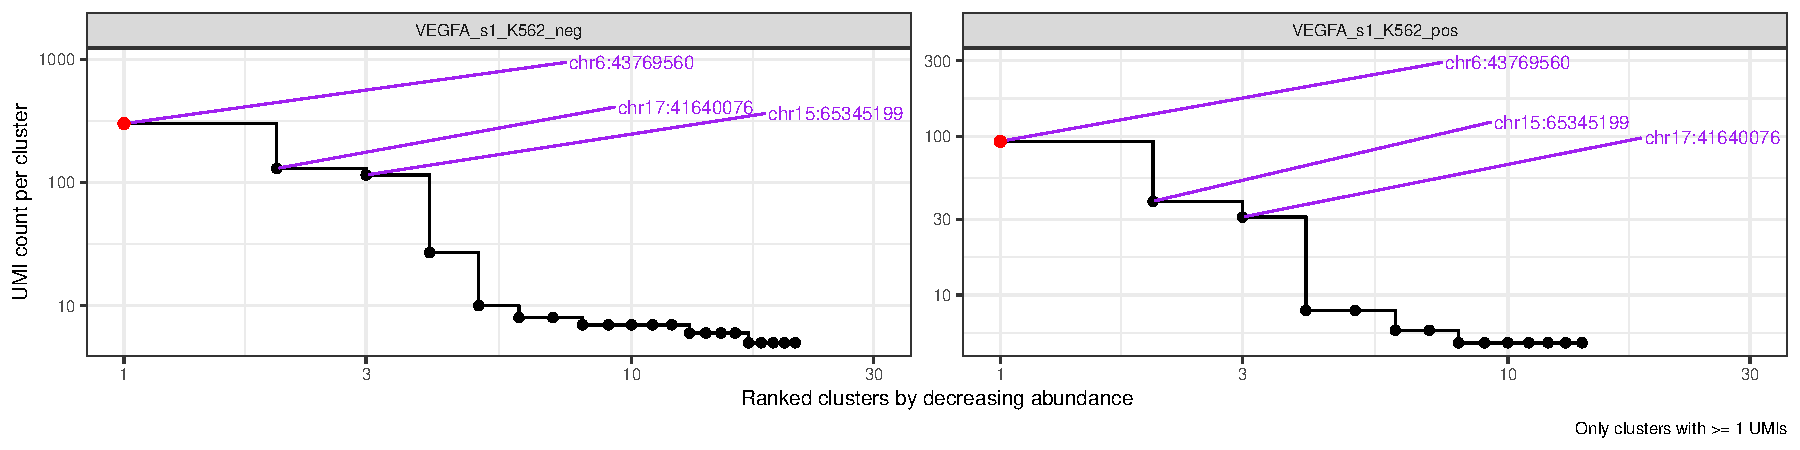
\includegraphics[width=0.9\linewidth]{/media/Data/common/guideseq_gnt_dev2/test_dataset/results/test_dataset_report_files/figure-latex/unnamed-chunk-6-1} 

}

\caption{Figure 1}\label{fig:unnamed-chunk-6}
\end{figure}

\begin{quote}
\begin{itemize}
\item
  Only clusters with gRNA match and more than \textbf{1} total UMIs are
  plotted.
\item
  \texttt{Red} dots correspond to clusters with \texttt{minimal\ edits}
  (see table 4).
\item
  Top3 most abundant clusters (UMI counts) are labeled.
\end{itemize}
\end{quote}

\subsection{Distribution of cut sites around best candidates
position}\label{distribution-of-cut-sites-around-best-candidates-position}

For each best candidate cluster, plot the UMI count detected around the
gRNA theoretical cut site (dashed line) for each cut site, in the
forward or reverse ODN orientation (blue and red bars respectively).

\begin{figure}[H]

{\centering 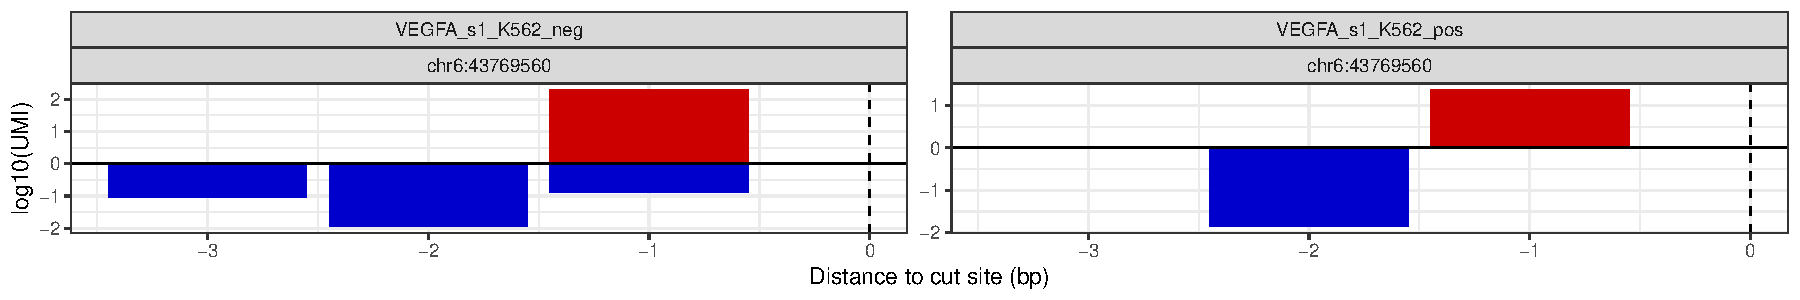
\includegraphics[width=0.9\linewidth]{/media/Data/common/guideseq_gnt_dev2/test_dataset/results/test_dataset_report_files/figure-latex/unnamed-chunk-7-1} 

}

\caption{Figure 2}\label{fig:unnamed-chunk-7}
\end{figure}

\section{Genome distribution of
clusters}\label{genome-distribution-of-clusters}

This figure represents the distribution of unique clusters
\texttt{with\ gRNA} match per chromosome, colored by \texttt{prediction}
status. Only clusters with number of edits (INDELs and substitutions)
smaller or equal to \textbf{6} are considered.

\begin{figure}[H]

{\centering 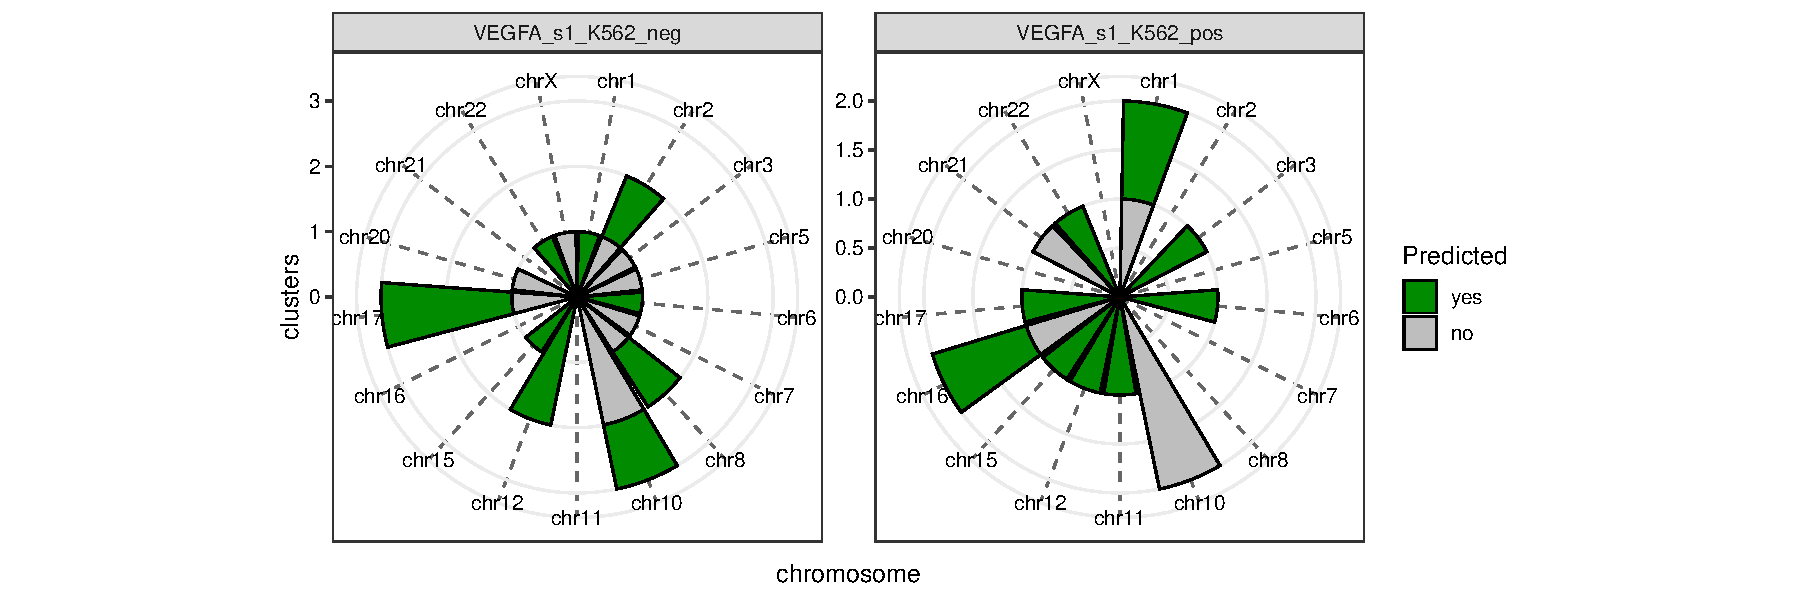
\includegraphics[width=0.9\linewidth]{/media/Data/common/guideseq_gnt_dev2/test_dataset/results/test_dataset_report_files/figure-latex/unnamed-chunk-8-1} 

}

\caption{figure 3}\label{fig:unnamed-chunk-8}
\end{figure}

This figure represents the total number of UMIs (cells) per chromosome
from clusters with gRNA match, colored by \texttt{prediction} status.
Only clusters with number of edits (INDELs and substitutions) smaller or
equal to \textbf{6} are considered.

\begin{figure}[H]

{\centering 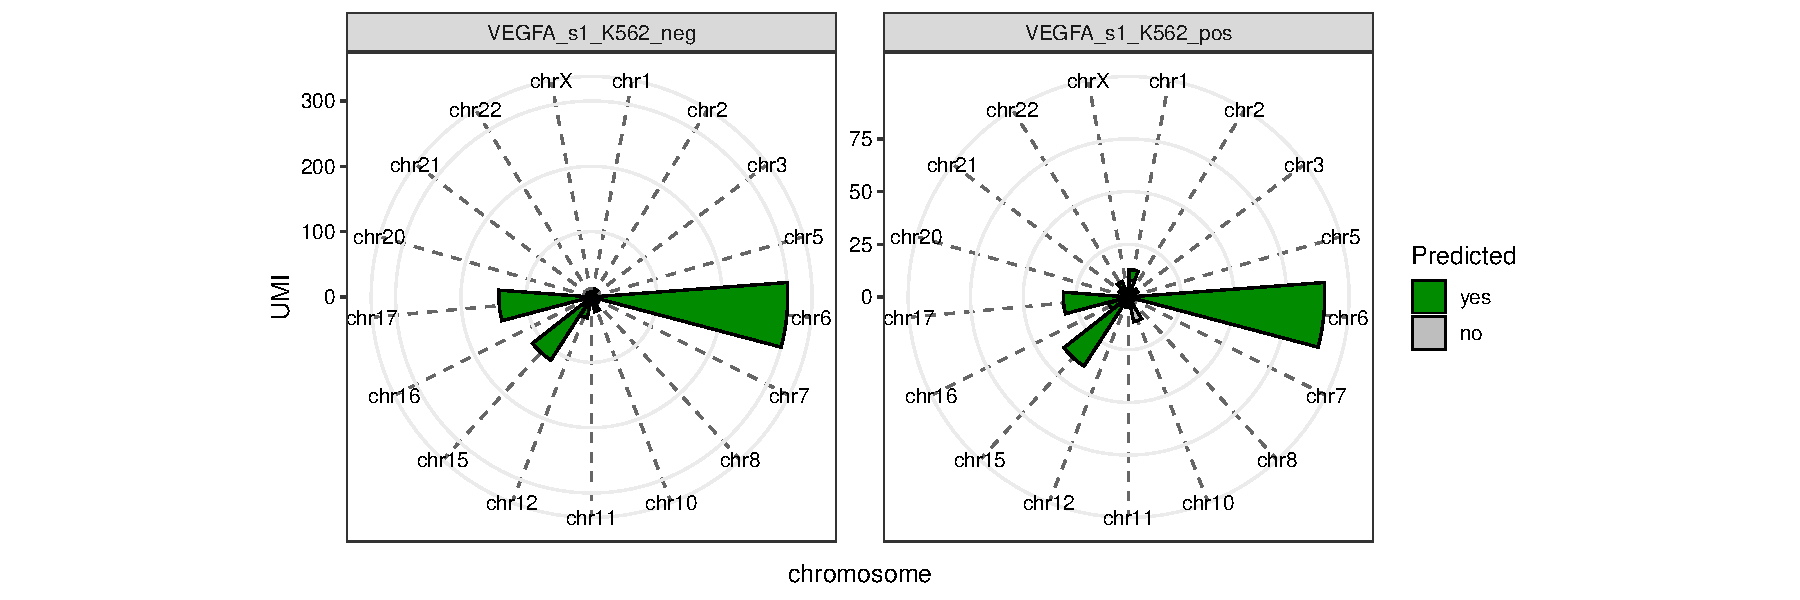
\includegraphics[width=0.9\linewidth]{/media/Data/common/guideseq_gnt_dev2/test_dataset/results/test_dataset_report_files/figure-latex/unnamed-chunk-9-1} 

}

\caption{figure 4}\label{fig:unnamed-chunk-9}
\end{figure}

\section{Configuration settings}\label{configuration-settings}

\begin{Shaded}
\begin{Highlighting}[]

\FunctionTok{author}\KeywordTok{:}\AttributeTok{ }\StringTok{"Guillaume CORRE, PhD"}
\FunctionTok{affiliation}\KeywordTok{:}\AttributeTok{ }\StringTok{"Therapeutic Gene Editing {-} GENETHON, INSERM U951, Paris{-}Saclay University, Evry, France"}
\FunctionTok{contact}\KeywordTok{:}\AttributeTok{ }\StringTok{"gcorre@genethon.fr"}
\FunctionTok{version}\KeywordTok{:}\AttributeTok{ }\StringTok{\textquotesingle{}V1.0\textquotesingle{}}

\FunctionTok{clean\_intermediates\_files}\KeywordTok{:}\AttributeTok{ }\StringTok{\textquotesingle{}TRUE\textquotesingle{}}

\CommentTok{\#\# Library informations}
\FunctionTok{sampleInfo\_path}\KeywordTok{:}\AttributeTok{ }\StringTok{"test\_datasheet.csv"}

\FunctionTok{read\_path}\KeywordTok{:}\AttributeTok{  }\StringTok{"./"}
\FunctionTok{R1}\KeywordTok{:}\AttributeTok{ }\StringTok{"Undetermined\_S0\_L001\_R1\_001.fastq.gz"}
\FunctionTok{R2}\KeywordTok{:}\AttributeTok{ }\StringTok{"Undetermined\_S0\_L001\_R2\_001.fastq.gz"}
\FunctionTok{I1}\KeywordTok{:}\AttributeTok{ }\StringTok{"Undetermined\_S0\_L001\_I1\_001.fastq.gz"}
\FunctionTok{I2}\KeywordTok{:}\AttributeTok{ }\StringTok{"Undetermined\_S0\_L001\_I2\_001.fastq.gz"}


\CommentTok{\#\#\#\#\#\#\#\#\#\#\#\#\#\#\#\#\#\#\#\#\#\#\#\#\#\#\#\#\#\#\#\#\#\#\#\#\#\#\#\#\#\#\#\#\#\#\#\#}
\CommentTok{\#\# path to references}
\FunctionTok{genome}\KeywordTok{:}
\AttributeTok{  }\FunctionTok{GRCh38}\KeywordTok{:}
\AttributeTok{    }\FunctionTok{fasta}\KeywordTok{:}\AttributeTok{ }\StringTok{"/media/References/Human/ensembl/GRCh38/Sequences/Homo\_sapiens.GRCh38.dna.primary\_assembly.fa"}
\AttributeTok{    }\FunctionTok{index}\KeywordTok{:}\AttributeTok{ }\StringTok{"/media/References/Human/ensembl/GRCh38/Indexes/Bowtie2/Homo\_sapiens.GRCh38.dna.primary\_assembly"}\CommentTok{ \# path to index created during the run if not existing yet}
\AttributeTok{    }\FunctionTok{annotation}\KeywordTok{:}\AttributeTok{ }\StringTok{"/media/References/Human/ensembl/GRCh38/Annotations/Homo\_sapiens.GRCh38.113.chr.gtf.gz"}
\AttributeTok{    }\FunctionTok{oncogene\_list}\KeywordTok{:}\AttributeTok{ }\StringTok{"/media/References/Human/ensembl/GRCh38/Annotations/OncoList\_OncoKB\_GRCh38\_2025{-}07{-}04.tsv"}
\AttributeTok{  }\FunctionTok{mouse}\KeywordTok{:}
\AttributeTok{    }\FunctionTok{fasta}\KeywordTok{:}\AttributeTok{ }\StringTok{""}
\AttributeTok{    }\FunctionTok{index}\KeywordTok{:}\AttributeTok{ }\StringTok{""}
\AttributeTok{    }\FunctionTok{annotation}\KeywordTok{:}\AttributeTok{ }\StringTok{""}
\CommentTok{\#\#\#\#\#\#\#\#\#\#\#\#\#\#\#\#\#\#\#\#\#\#\#\#\#\#\#\#\#\#\#\#\#\#\#\#\#\#\#\#\#\#\#\#\#\#\#\#}

\CommentTok{\#\#\#\#\#\#\#\#\#\#\#\#\#\#\#\#\#\#\#\#\#\#\#\#\#\#\#\#\#\#\#\#\#\#\#\#\#\#\#\#\#\#\#\#\#\#\#\#}
\FunctionTok{minLength}\KeywordTok{:}\AttributeTok{ }\DecValTok{25}\CommentTok{ \#\# Minimal read length after trimming, before alignment}
\CommentTok{\#\#\#\#\#\#\#\#\#\#\#\#\#\#\#\#\#\#\#\#\#\#\#\#\#\#\#\#\#\#\#\#\#\#\#\#\#\#\#\#\#\#\#\#\#\#\#\#}

\CommentTok{\#\# Alignement }
\CommentTok{\#\#\#\#\#\#\#\#\#\#\#\#\#\#\#\#\#\#\#\#\#\#\#\#\#\#\#\#\#\#\#\#\#\#\#\#\#\#\#\#\#\#\#\#\#\#\#\#}
\FunctionTok{aligner}\KeywordTok{:}\AttributeTok{ }\StringTok{"bowtie2"}\CommentTok{   \#\# Aligner to use (bowtie2 or bwa)}
\FunctionTok{minFragLength}\KeywordTok{:}\AttributeTok{ }\DecValTok{100}\CommentTok{         \# Minimal fragment length after alignment}
\FunctionTok{maxFragLength}\KeywordTok{:}\AttributeTok{ }\DecValTok{1500}\CommentTok{        \# Maximal fragment length after alignment }
\FunctionTok{rescue\_R2}\KeywordTok{:}\AttributeTok{ }\StringTok{"TRUE"}\CommentTok{     \# Rescur R2 reads if R1 is too short or the pair doesn\textquotesingle{}t align properly.}

\CommentTok{\#\#\#\#\#\#\#\#\#\#\#\#\#\#\#\#\#\#\#\#\#\#\#\#\#\#\#\#\#\#\#\#\#\#\#\#\#\#\#\#\#\#\#\#\#\#\#\#}

\CommentTok{\#\#\#\#\#\#\#\#\#\#\#\#\#\#\#\#\#\#\#\#\#\#\#\#\#\#\#\#\#\#\#\#\#\#\#\#\#\#\#\#\#\#\#\#\#\#\#\#}
\CommentTok{\# post alignment}
\FunctionTok{minMAPQ}\KeywordTok{:}\AttributeTok{ }\DecValTok{20}\CommentTok{                      \# Min MAPQ score to keep alignments }
\FunctionTok{UMI\_hamming\_distance}\KeywordTok{:}\AttributeTok{ }\DecValTok{1}\CommentTok{         \# min distance to cluster UMI using network{-}based deduplication, use [0] to keep raw UMIs}
\FunctionTok{UMI\_deduplication}\KeywordTok{:}\AttributeTok{ }\StringTok{"Adjacency"}\CommentTok{  \# method to correct UMI (cluster or Adjacency)}
\FunctionTok{UMI\_pattern}\KeywordTok{:}\AttributeTok{ }\StringTok{"NNWNNWNN"}\AttributeTok{  }
\FunctionTok{UMI\_filter}\KeywordTok{:}\AttributeTok{ }\StringTok{"TRUE"}\CommentTok{              \# If TRUE, remove UMIs that do no match the expected pattern [FALSE or TRUE]}
\CommentTok{\#\#\#\#\#\#\#\#\#\#\#\#\#\#\#\#\#\#\#\#\#\#\#\#\#\#\#\#\#\#\#\#\#\#\#\#\#\#\#\#\#\#\#\#\#\#\#\#}


\CommentTok{\#\#\#\#\#\#\#\#\#\#\#\#\#\#\#\#\#\#\#\#\#\#\#\#\#\#\#\#\#\#\#\#\#\#\#\#\#\#\#\#\#\#\#\#\#\#\#\#}
\CommentTok{\#\# Off targets calling}
\FunctionTok{tolerate\_bulges}\KeywordTok{:}\AttributeTok{ }\StringTok{"TRUE"}\CommentTok{           \# whether to include gaps in the gRNA alignment (this will change the gap penalty during SW pairwise alignment)}
\FunctionTok{max\_edits\_crRNA}\KeywordTok{:}\AttributeTok{ }\DecValTok{6}\CommentTok{                \# filter clusters with less or equal than n edits in the crRNA sequence (edits = substitutions + INDELs)}
\FunctionTok{ISbinWindow}\KeywordTok{:}\AttributeTok{ }\DecValTok{100}\CommentTok{                  \# insertion sites closer than \textquotesingle{}ISbinWindow\textquotesingle{} will be clustered together}
\FunctionTok{minReadsPerUMI}\KeywordTok{:}\AttributeTok{ }\DecValTok{4}\CommentTok{                 \# Min number of reads per UMIs (\textgreater{}=)}
\FunctionTok{minUMIPerIS}\KeywordTok{:}\AttributeTok{ }\DecValTok{4}\CommentTok{                      \# Min number of UMI per IS (\textgreater{}=)}
\FunctionTok{slopSize}\KeywordTok{:}\AttributeTok{ }\DecValTok{50}\CommentTok{                      \# window size (bp) around IS (both directions) to identify gRNA sequence (ie 50bp = {-}50bp to +50bp)}
\FunctionTok{min\_predicted\_distance}\KeywordTok{:}\AttributeTok{ }\DecValTok{100}\CommentTok{       \# distance between cut site and predicted cut site to consider as predicted}
\CommentTok{\#\#\#\#\#\#\#\#\#\#\#\#\#\#\#\#\#\#\#\#\#\#\#\#\#\#\#\#\#\#\#\#\#\#\#\#\#\#\#\#\#\#\#\#\#\#\#\#}

\CommentTok{\#\#\#\#\#\#\#\#\#\#\#\#\#\#\#\#\#\#\#\#\#\#\#\#\#\#\#\#\#\#\#\#\#\#\#\#\#\#\#\#\#\#\#\#\#\#\#\#}
\CommentTok{\# reporting}
\FunctionTok{max\_clusters}\KeywordTok{:}\AttributeTok{ }\DecValTok{100}\CommentTok{                 \# max number of cluster alignments to report}
\FunctionTok{minUMI\_alignments\_figure}\KeywordTok{:}\AttributeTok{ }\DecValTok{1}\CommentTok{       \# filter clusters with more than n UMI in the report alignment figure (set to 0 to keep all clusters {-}\textgreater{} can be slow)}
\CommentTok{\#\#\#\#\#\#\#\#\#\#\#\#\#\#\#\#\#\#\#\#\#\#\#\#\#\#\#\#\#\#\#\#\#\#\#\#\#\#\#\#\#\#\#\#\#\#\#\#}

\CommentTok{\# Prediction}
\CommentTok{\#\#\#\#\#\#\#\#\#\#\#\#\#\#\#\#\#\#\#\#\#\#\#\#\#\#\#\#\#\#\#\#\#\#\#\#\#\#\#\#\#\#\#\#\#\#\#\#}
\FunctionTok{SWoffFinder}\KeywordTok{:}
\AttributeTok{  }\FunctionTok{path}\KeywordTok{:}\AttributeTok{ }\StringTok{"/opt/SWOffinder"}\CommentTok{ \#\# Path to SWoffinder on your server (downloaded from https://github.com/OrensteinLab/SWOffinder)}
\AttributeTok{  }\FunctionTok{maxE}\KeywordTok{:}\AttributeTok{ }\DecValTok{6}\CommentTok{                 \# Max edits allowed (integer).}
\AttributeTok{  }\FunctionTok{maxM}\KeywordTok{:}\AttributeTok{ }\DecValTok{6}\CommentTok{                 \# Max mismatches allowed without bulges (integer).}
\AttributeTok{  }\FunctionTok{maxMB}\KeywordTok{:}\AttributeTok{ }\DecValTok{6}\CommentTok{                \# Max mismatches allowed with bulges (integer).}
\AttributeTok{  }\FunctionTok{maxB}\KeywordTok{:}\AttributeTok{ }\DecValTok{3}\CommentTok{                 \# Max bulges allowed (integer).}
\AttributeTok{  }\FunctionTok{window\_size}\KeywordTok{:}\AttributeTok{ }\DecValTok{100}
\CommentTok{\#\#\#\#\#\#\#\#\#\#\#\#\#\#\#\#\#\#\#\#\#\#\#\#\#\#\#\#\#\#\#\#\#\#\#\#\#\#\#\#\#\#\#\#\#\#\#\#}



\CommentTok{\#\#\#\#\#\#\#\#\#\#\#\#\#\#\#\#\#\#\#\#\#\#\#\#\#\#\#\#\#\#\#\#\#\#\#\#\#\#\#\#\#\#\#\#\#\#\#\#}
\CommentTok{\# Sequences for the trimming steps}

\FunctionTok{guideseq}\KeywordTok{:}
\AttributeTok{  }\FunctionTok{positive}\KeywordTok{:}
\AttributeTok{    }\FunctionTok{R1\_trailing}\KeywordTok{:}\AttributeTok{ }\StringTok{"GTTTAATTGAGTTGTCATATGT"}
\AttributeTok{    }\FunctionTok{R2\_leading}\KeywordTok{:}\AttributeTok{ }\StringTok{"ACATATGACAACTCAATTAAAC"}
\AttributeTok{    }\FunctionTok{R2\_trailing}\KeywordTok{:}\AttributeTok{ }\StringTok{"AGATCGGAAGAGCGTCGTGT"}
\AttributeTok{  }\FunctionTok{negative}\KeywordTok{:}
\AttributeTok{    }\FunctionTok{R1\_trailing}\KeywordTok{:}\AttributeTok{ }\StringTok{"ATACCGTTATTAACATATGACAACTCAA"}
\AttributeTok{    }\FunctionTok{R2\_leading}\KeywordTok{:}\AttributeTok{ }\StringTok{"TTGAGTTGTCATATGTTAATAACGGTAT"}
\AttributeTok{    }\FunctionTok{R2\_trailing}\KeywordTok{:}\AttributeTok{ }\StringTok{"AGATCGGAAGAGCGTCGTGT"}



\FunctionTok{iguideseq}\KeywordTok{:}
\AttributeTok{  }\FunctionTok{positive}\KeywordTok{:}
\AttributeTok{    }\FunctionTok{R2\_leading}\KeywordTok{:}\AttributeTok{ }\StringTok{"ACATATGACAACTCAATTAAACGCGAGC"}
\AttributeTok{    }\FunctionTok{R2\_trailing}\KeywordTok{:}\AttributeTok{ }\StringTok{"AGATCGGAAGAGCGTCGTGT"}
\AttributeTok{    }\FunctionTok{R1\_trailing}\KeywordTok{:}\AttributeTok{ }\StringTok{"GCTCGCGTTTAATTGAGTTGTCATATGT"}
\AttributeTok{  }\FunctionTok{negative}\KeywordTok{:}
\AttributeTok{    }\FunctionTok{R1\_trailing}\KeywordTok{:}\AttributeTok{ }\StringTok{"TCGCGTATACCGTTATTAACATATGACAACTCAA"}
\AttributeTok{    }\FunctionTok{R2\_leading}\KeywordTok{:}\AttributeTok{ }\StringTok{"TTGAGTTGTCATATGTTAATAACGGTATACGCGA"}
\AttributeTok{    }\FunctionTok{R2\_trailing}\KeywordTok{:}\AttributeTok{ }\StringTok{"AGATCGGAAGAGCGTCGTGT"}
\AttributeTok{    }
\AttributeTok{    }
\AttributeTok{    }
\FunctionTok{olitagseq}\KeywordTok{:}
\AttributeTok{  }\FunctionTok{positive}\KeywordTok{:}
\AttributeTok{    }\FunctionTok{R1\_trailing}\KeywordTok{:}\AttributeTok{ }\StringTok{"GGGGTTTAATTGAGTTGTCATATGTT"}
\AttributeTok{    }\FunctionTok{R2\_leading}\KeywordTok{:}\AttributeTok{ }\StringTok{"AACATATGACAACTCAATTAAACCCC"}
\AttributeTok{    }\FunctionTok{R2\_trailing}\KeywordTok{:}\AttributeTok{ }\StringTok{"TCCGCTCCCTCG"}
\AttributeTok{  }\FunctionTok{negative}\KeywordTok{:}
\AttributeTok{    }\FunctionTok{R1\_trailing}\KeywordTok{:}\AttributeTok{ }\StringTok{"CCCATACCGTTATTAACATATGAC"}
\AttributeTok{    }\FunctionTok{R2\_leading}\KeywordTok{:}\AttributeTok{ }\StringTok{"GTCATATGTTAATAACGGTATGGG"}
\AttributeTok{    }\FunctionTok{R2\_trailing}\KeywordTok{:}\AttributeTok{ }\StringTok{"TCCGCTCCCTCG"}

\FunctionTok{tagseq}\KeywordTok{:}
\AttributeTok{  }\FunctionTok{positive}\KeywordTok{:}
\AttributeTok{    }\FunctionTok{R1\_trailing}\KeywordTok{:}\AttributeTok{ }\StringTok{"TGCGATAACACGCATTTCGCATAA"}
\AttributeTok{    }\FunctionTok{R2\_leading}\KeywordTok{:}\AttributeTok{ }\StringTok{"CTTATGCGAAATGCGTGTTATCGCA"}
\AttributeTok{    }\FunctionTok{R2\_trailing}\KeywordTok{:}\AttributeTok{ }\StringTok{"AGATCGGAAGAGCGTCGTGT"}
\AttributeTok{  }\FunctionTok{negative}\KeywordTok{:}
\AttributeTok{    }\FunctionTok{R1\_trailing}\KeywordTok{:}\AttributeTok{ }\StringTok{"ATCTCTGAGCCTTATGCGAAATGC"}
\AttributeTok{    }\FunctionTok{R2\_leading}\KeywordTok{:}\AttributeTok{ }\StringTok{"CGCATTTCGCATAAGGCTCAGAGAT"}
\AttributeTok{    }\FunctionTok{R2\_trailing}\KeywordTok{:}\AttributeTok{ }\StringTok{"AGATCGGAAGAGCGTCGTGT"}
\CommentTok{\#\#\#\#\#\#\#\#\#\#\#\#\#\#\#\#\#\#\#\#\#\#\#\#\#\#\#\#\#\#\#\#\#\#\#\#\#\#\#\#\#\#\#\#\#\#\#\#}
\end{Highlighting}
\end{Shaded}

\section{R session informations}\label{r-session-informations}

R version 4.4.3 (2025-02-28) Platform: x86\_64-conda-linux-gnu Running
under: Debian GNU/Linux 12 (bookworm)

Matrix products: default BLAS/LAPACK:
/opt/miniconda/envs/guideseq/lib/libopenblasp-r0.3.30.so; LAPACK version
3.12.0

locale: {[}1{]} LC\_CTYPE=fr\_FR.UTF-8 LC\_NUMERIC=C\\
{[}3{]} LC\_TIME=fr\_FR.UTF-8 LC\_COLLATE=fr\_FR.UTF-8\\
{[}5{]} LC\_MONETARY=fr\_FR.UTF-8 LC\_MESSAGES=fr\_FR.UTF-8\\
{[}7{]} LC\_PAPER=fr\_FR.UTF-8 LC\_NAME=C\\
{[}9{]} LC\_ADDRESS=C LC\_TELEPHONE=C\\
{[}11{]} LC\_MEASUREMENT=fr\_FR.UTF-8 LC\_IDENTIFICATION=C

time zone: Europe/Paris tzcode source: system (glibc)

attached base packages: {[}1{]} stats graphics grDevices utils datasets
methods base

other attached packages: {[}1{]} UpSetR\_1.4.0 yaml\_2.3.10
kableExtra\_1.4.0 lubridate\_1.9.4 {[}5{]} forcats\_1.0.1 stringr\_1.5.2
dplyr\_1.1.4 purrr\_1.1.0\\
{[}9{]} readr\_2.1.5 tidyr\_1.3.1 tibble\_3.3.0 ggplot2\_4.0.0\\
{[}13{]} tidyverse\_2.0.0 rmdformats\_1.0.4

loaded via a namespace (and not attached): {[}1{]} generics\_0.1.4
xml2\_1.4.0 stringi\_1.8.7 hms\_1.1.3\\
{[}5{]} digest\_0.6.37 magrittr\_2.0.4 evaluate\_1.0.5 grid\_4.4.3\\
{[}9{]} timechange\_0.3.0 RColorBrewer\_1.1-3 bookdown\_0.44
fastmap\_1.2.0\\
{[}13{]} plyr\_1.8.9 ggrepel\_0.9.6 gridExtra\_2.3 viridisLite\_0.4.2
{[}17{]} scales\_1.4.0 textshaping\_1.0.3 cli\_3.6.5 rlang\_1.1.6\\
{[}21{]} withr\_3.0.2 tools\_4.4.3 tzdb\_0.5.0 vctrs\_0.6.5\\
{[}25{]} R6\_2.6.1 lifecycle\_1.0.4 pkgconfig\_2.0.3 pillar\_1.11.1\\
{[}29{]} gtable\_0.3.6 glue\_1.8.0 Rcpp\_1.1.0 systemfonts\_1.3.1
{[}33{]} xfun\_0.53 tidyselect\_1.2.1 rstudioapi\_0.17.1 knitr\_1.50\\
{[}37{]} farver\_2.1.2 htmltools\_0.5.8.1 labeling\_0.4.3
rmarkdown\_2.30\\
{[}41{]} svglite\_2.2.1 compiler\_4.4.3 S7\_0.2.0

\end{document}
